% $Header: /cvsroot/latex-beamer/latex-beamer/solutions/conference-talks/conference-ornate-20min.en.tex,v 1.6 2004/10/07 20:53:08 tantau Exp $

\documentclass{beamer}
%\documentclass[handout]{beamer}
%\usepackage{pgfpages}
%\pgfpagesuselayout{2 on 1}[a4paper,border shrink=5mm]

% This file is a solution template for:

% - Talk at a conference/colloquium.
% - Talk length is about 20min.
% - Style is ornate.



% Copyright 2004 by Till Tantau <tantau@users.sourceforge.net>.
%
% In principle, this file can be redistributed and/or modified under
% the terms of the GNU Public License, version 2.
%
% However, this file is supposed to be a template to be modified
% for your own needs. For this reason, if you use this file as a
% template and not specifically distribute it as part of a another
% package/program, I grant the extra permission to freely copy and
% modify this file as you see fit and even to delete this copyright
% notice.


\mode<presentation>
{
%  \usetheme{Warsaw}
%  \usetheme{Boadilla}
%  \usetheme{Goettingen}
%  \usetheme{Hannover}
%  \usetheme{Madrid}
%  \usetheme{Marburg}
%  \usetheme{Montpellier}
%  \usetheme{Pittsburgh}
  \usetheme{Hawke}
  % or ...

  \setbeamercovered{transparent}
  % or whatever (possibly just delete it)
}


\usepackage[english]{babel}
% or whatever

\usepackage[latin1]{inputenc}
% or whatever

\usepackage{times}
\usepackage[T1]{fontenc}
% Or whatever. Note that the encoding and the font should match. If T1
% does not look nice, try deleting the line with the fontenc.

\usepackage{multimedia}


%%%%%%
% My Commands
%%%%%%

\newcommand{\ml}{{\sc matlab}}
\newcommand{\bb}{{\boldsymbol{b}}}
\newcommand{\bx}{{\boldsymbol{x}}}
\newcommand{\by}{{\boldsymbol{y}}}
\newcommand{\bfm}[1]{{\boldsymbol{#1}}}

%%%%

\title[Lecture 15] % (optional, use only with long paper titles)
{Lecture 15 - Initial Value Problems}

% \subtitle
% {Include Only If Paper Has a Subtitle}

\author[I. Hawke] % (optional, use only with lots of authors)
{I.~Hawke}
% - Give the names in the same order as the appear in the paper.
% - Use the \inst{?} command only if the authors have different
%   affiliation.

\institute[University of Southampton] % (optional, but mostly needed)
{
%  \inst{1}%
  School of Mathematics, \\
  University of Southampton, UK
}
% - Use the \inst command only if there are several affiliations.
% - Keep it simple, no one is interested in your street address.

\date[Semester 1] % (optional, should be abbreviation of conference name)
{MATH3018/6141, Semester 1}
% - Either use conference name or its abbreviation.
% - Not really informative to the audience, more for people (including
%   yourself) who are reading the slides online

\subject{Numerical methods}
% This is only inserted into the PDF information catalog. Can be left
% out.



% If you have a file called "university-logo-filename.xxx", where xxx
% is a graphic format that can be processed by latex or pdflatex,
% resp., then you can add a logo as follows:

\pgfdeclareimage[height=0.5cm]{university-logo}{mathematics_7469}
\logo{\pgfuseimage{university-logo}}



% Delete this, if you do not want the table of contents to pop up at
% the beginning of each subsection:
%  \AtBeginSubsection[]
%  {
%    \begin{frame}<beamer>
%      \frametitle{Outline}
%      \tableofcontents[currentsection,currentsubsection]
%    \end{frame}
%  }
\AtBeginSection[]
{
  \begin{frame}<beamer>
    \frametitle{Outline}
    \tableofcontents[currentsection]
  \end{frame}
}


% If you wish to uncover everything in a step-wise fashion, uncomment
% the following command:

%\beamerdefaultoverlayspecification{<+->}


\begin{document}

\begin{frame}
  \titlepage
\end{frame}

\section{Predictor-Corrector methods}

\subsection{Predictor-Corrector methods}

\begin{frame}
  \frametitle{Geometrical interpretation of Euler's method}

  Considering IVPs in the form
  \begin{equation*}
    \by'(x) = \bfm{f}(x, \by(x)).
  \end{equation*}

  The simple (first order accurate, explicit) Euler method is
  \begin{equation*}
    \by_{n+1} = \by_n + h \bfm{f}(x_n, \by_n).
  \end{equation*} \pause

  Euler's method is not sufficiently accurate for practical use. The
  geometrical interpretation is that the slope ($\by'$) over the
  interval $[x_n, x_{n+1}]$ is approximated by the slope at the
  \emph{beginning} of the interval,
  \begin{equation*}
    \by' \simeq \by'(x_n).
  \end{equation*} \pause

  Try a better approximation to the slope for a more accurate result.

\end{frame}

\begin{frame}
  \frametitle{Predicting and correcting}

  \begin{overlayarea}{\textwidth}{0.8\textheight}
    \only<1-3|handout:1>
    {
      Still using forward differencing for $\by'$, an ``average''
      slope is
      \begin{equation*}
        \frac{\by_{n+1} - \by_n}{h} = \frac{\bfm{f}(x_n, \by_n) +
          \bfm{f}(x_{n+1}, \by_{n+1})}{2}.
      \end{equation*}
    }
    \only<2-3|handout:1>
    {
      Rearrange: gives the unknown $\by_{n+1}$ as
      \begin{equation*}
        \by_{n+1} = \by_n + \frac{h}{2} \left( \bfm{f}(x_n, \by_n) +
          \bfm{f}(x_{n+1}, \by_{n+1}) \right).
      \end{equation*}
    }
    \only<3|handout:1>
    {
      But we need $\by_{n+1}$ to compute the right-hand-side.
    }
    \only<4-|handout:2>
    {
      \begin{equation*}
        \by_{n+1} = \by_n + \frac{h}{2} \left( \bfm{f}(x_n, \by_n) +
          \bfm{f}(x_{n+1}, \by_{n+1}) \right).
      \end{equation*}

      \vspace{1ex}

      Instead compute a \emph{guess} for $\by_{n+1}$, and use this
      guess when required. This is the \emph{predictor} step:
      \begin{equation*}
        \by_{n+1}^{(p)} = \by_n + h \bfm{f}(x_n, \by_n)
      \end{equation*}
      if we use Euler's method for the prediction.
    }
    \only<5-|handout:2>
    {

      \vspace{1ex}
      Using this, apply the \emph{corrector} step
      \begin{equation*}
        \by_{n+1} = \by_n + \frac{h}{2} \left( \bfm{f}(x_n, \by_n) +
          \bfm{f}(x_{n+1}, \by_{n+1}^{(p)}) \right),
      \end{equation*}
      which describes the (Euler) \emph{predictor-corrector} method.
    }
    \only<6|handout:2>
    {

      \vspace{1ex}
      The \emph{local} error is $\propto {\cal O}(h^3)$.
    }
  \end{overlayarea}

\end{frame}

\begin{frame}
  \frametitle{Example}


  Apply the Euler predictor-corrector method to
  \begin{equation*}
    y'(x) = - \sin(x), \quad y(0) = 1
  \end{equation*}
  to integrate up to $x = 0.5$. With $h = 0.1$:
  \begin{center}
    \begin{tabular}{c|c c c c c c}
      $n$ & $x_n$ & $y_n$ & $f(x_n, y_n)$ & $y_{n+1}^{(p)}$ & $f(x_{n+1},
      y_{n+1}^{(p)})$ & $\cos(x_n)$ \\
      \hline
      0 & 0.0 & 1.000 &  0.000 & 1.000 & -0.100 & 1.000 \\
      1 & 0.1 & 0.995 & -0.100 & 0.985 & -0.199 & 0.995 \\
      2 & 0.2 & 0.980 & -0.199 & 0.960 & -0.296 & 0.980 \\
      3 & 0.3 & 0.955 & -0.296 & 0.926 & -0.389 & 0.955 \\
      4 & 0.4 & 0.921 & -0.389 & 0.882 & -0.479 & 0.921 \\
      5 & 0.5 & 0.878 &        &       &        & 0.878
    \end{tabular}
  \end{center} \pause
  The error is $0.1\%$, not visible at this precision. With $h = 0.01$
  then the error is $0.001\%$, showing second order convergence.

\end{frame}


\begin{frame}
  \frametitle{Example: 2}


  Consider the system
  \begin{equation*}
    \left\{
      \begin{aligned}
        \dot{x} & = -y \\ \dot{y} & = x
      \end{aligned} \right., \quad x(0) = 1, \, \, y(0) = 0.
  \end{equation*}
  In polar coordinates this is $\dot{r} = 0$, $\dot{\phi} = 1$.
  \begin{columns}
    \begin{column}{0.5\textwidth}
      \begin{overlayarea}{\textwidth}{0.4\textheight}
        \only<2-3|handout:1>
        {
          Use the predictor-corrector method with $h=0.1$. At $t=500$
          the result matches the correct answer to the eye.
        }
        \only<3|handout:1>
        {

          \vspace{1ex}
          The growth of the radius makes the errors visible.
        }
        \only<4-5|handout:2>
        {
          Use the predictor-corrector method with $h=0.01$. At $t=500$
          the result matches the correct answer to the eye.
        }
        \only<5|handout:2>
        {

          \vspace{1ex}
          Looking at the growth of the radius makes the errors
          visible even now.
        }
      \end{overlayarea}
    \end{column}
    \begin{column}{0.5\textwidth}
      \begin{overlayarea}{\textwidth}{0.6\textheight}
        \only<2|handout:0>
        {
          \begin{center}
            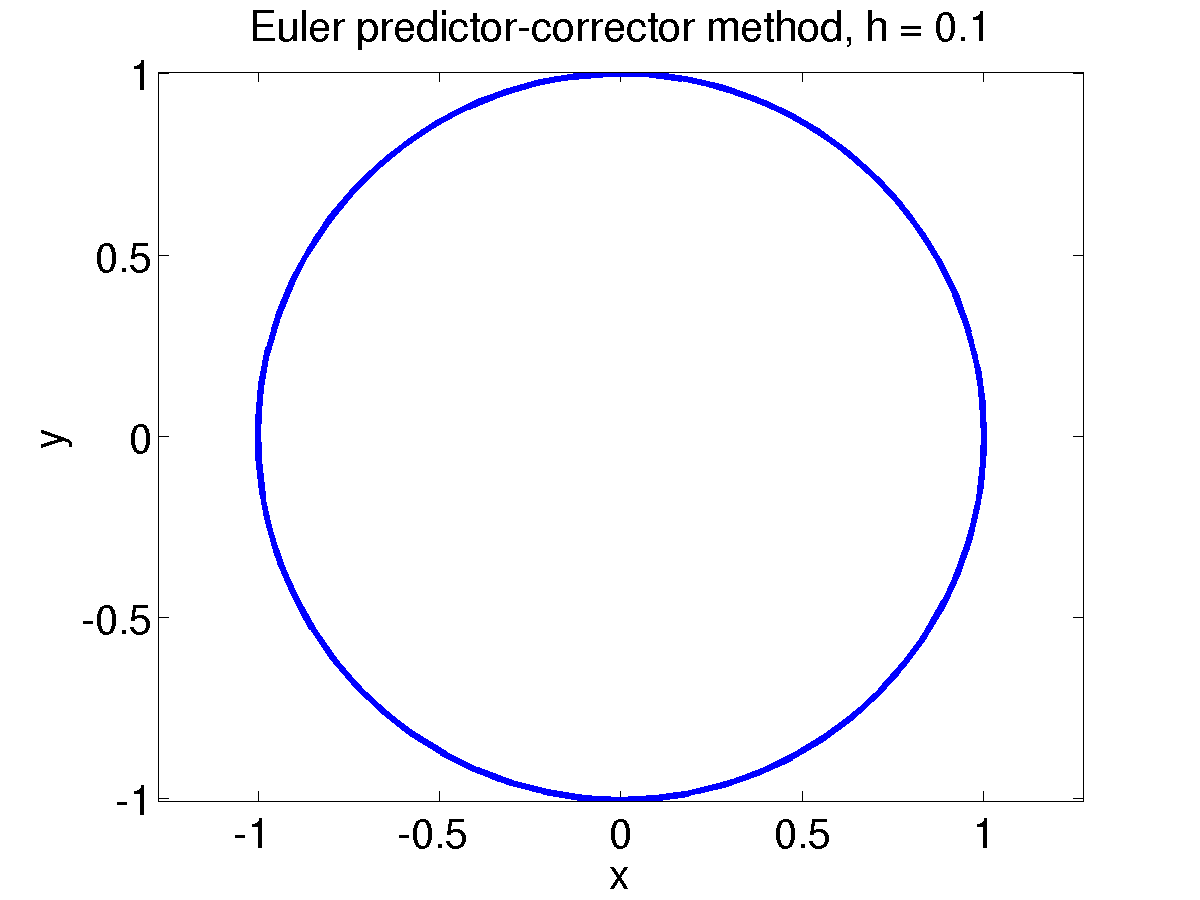
\includegraphics[height=0.5\textheight]{figures/EulerPC1}
          \end{center}
        }
        \only<3|handout:1>
        {
          \begin{center}
            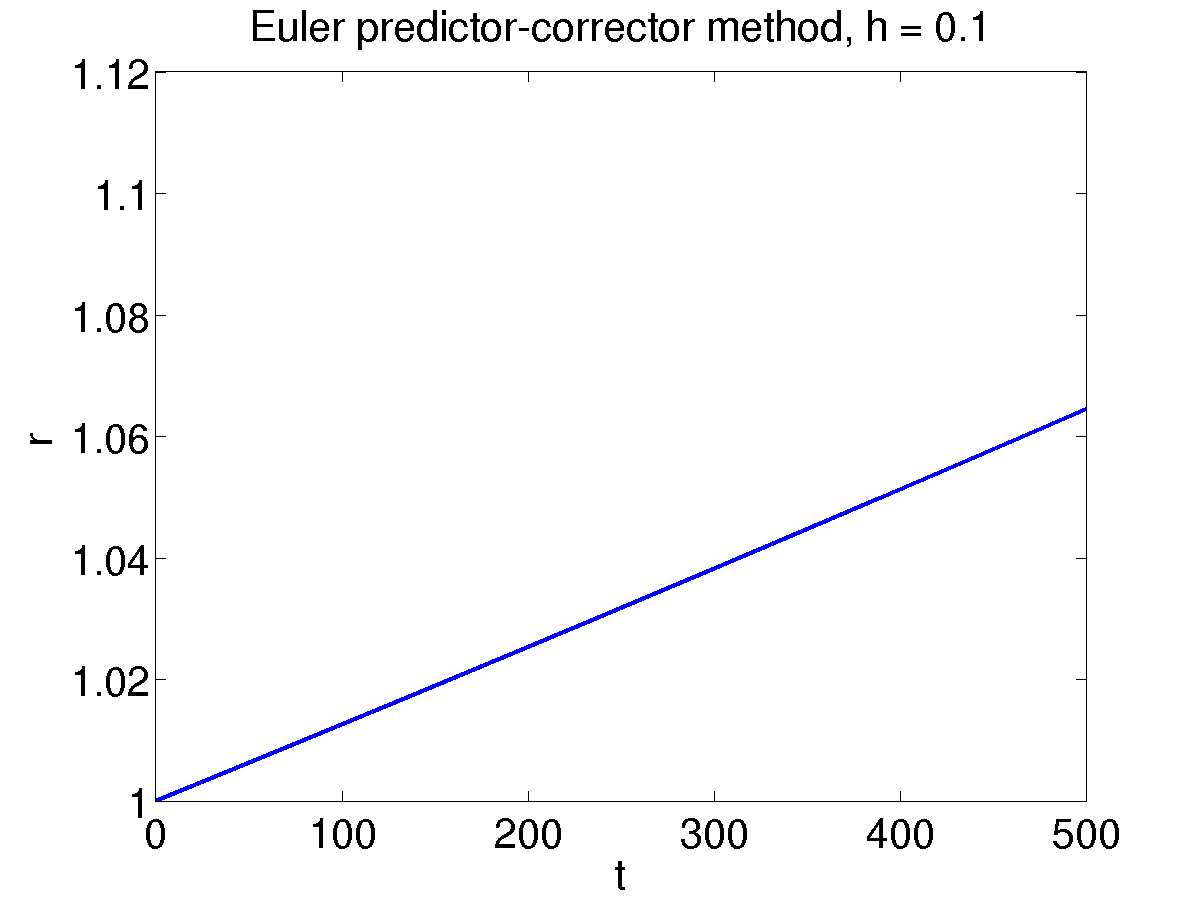
\includegraphics[height=0.5\textheight]{figures/EulerPC_rad1}
          \end{center}
        }
        \only<4|handout:0>
        {
          \begin{center}
            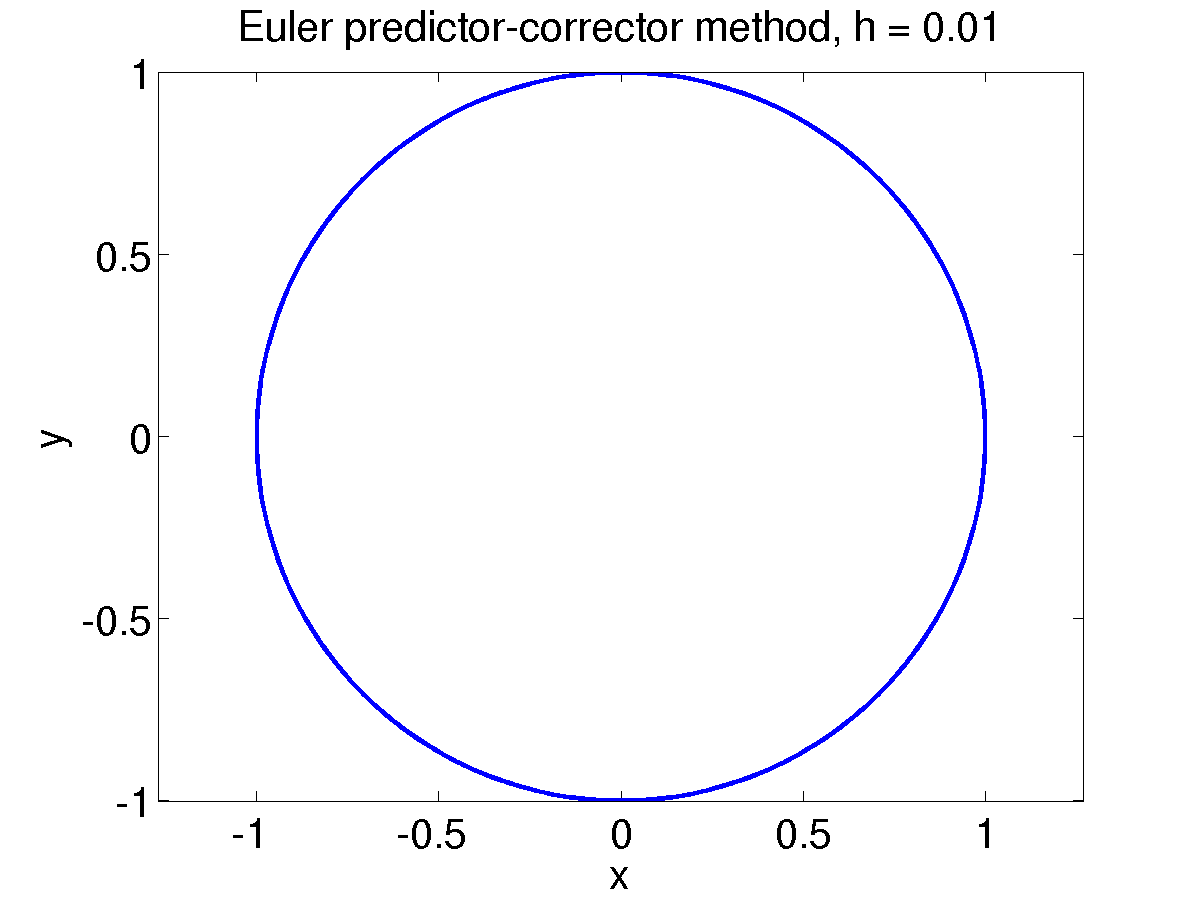
\includegraphics[height=0.5\textheight]{figures/EulerPC2}
          \end{center}
        }
        \only<5|handout:2>
        {
          \begin{center}
            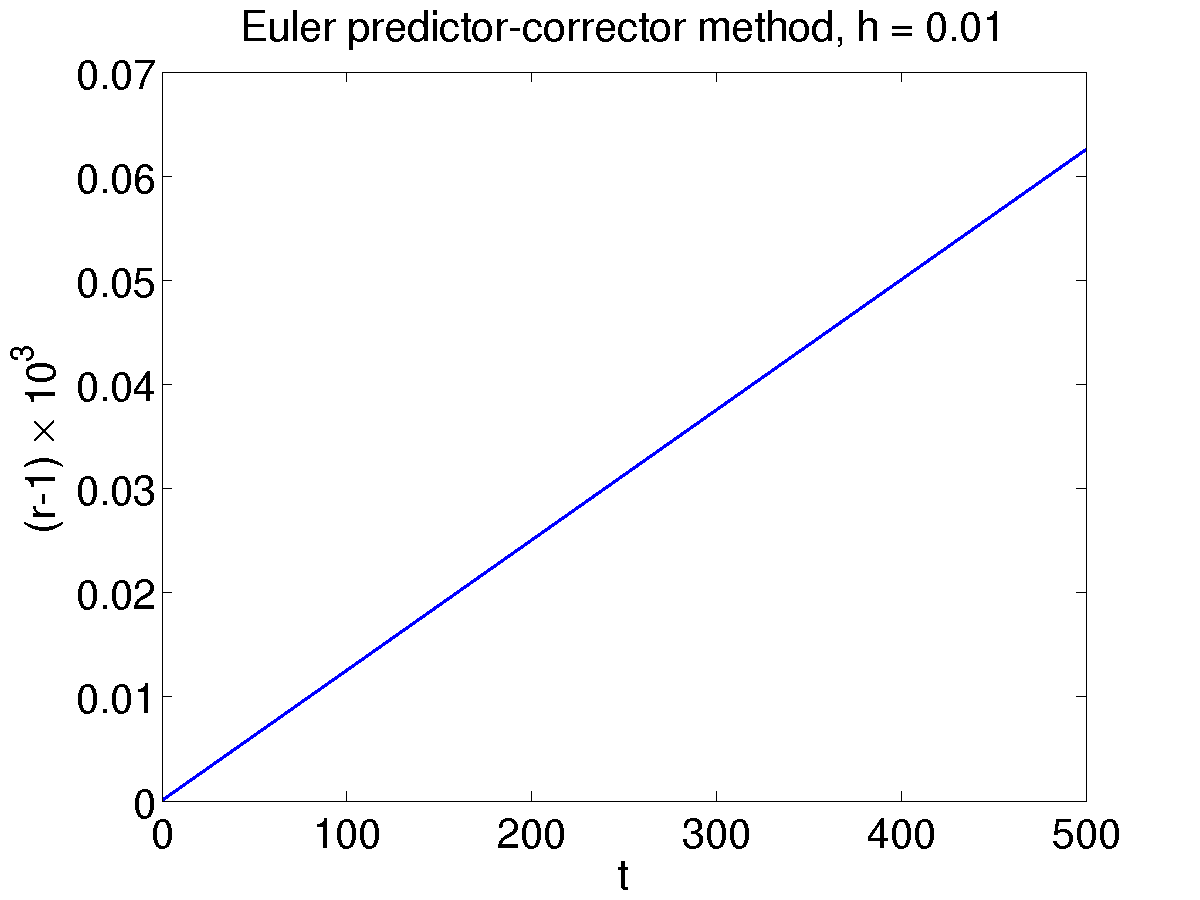
\includegraphics[height=0.5\textheight]{figures/EulerPC_rad2}
          \end{center}
        }
      \end{overlayarea}
    \end{column}
  \end{columns}

\end{frame}


\section{Errors}

\subsection{Errors}

\begin{frame}
  \frametitle{Errors}


  \begin{columns}
    \begin{column}{0.5\textwidth}
      With quadrature using e.g.\ Simpson's rule the \emph{local}
      error on any subinterval gave
      \begin{equation*}
        |{\cal E}_{\text{global}}| \le \sum |{\cal E}_{\text{local}}|.
      \end{equation*} \pause

      For an IVP we still have the \emph{local} and \emph{global}
      errors.  But steps are not independent so the error bound is
      different.
    \end{column}
    \begin{column}{0.5\textwidth}
      \begin{center}
        \includegraphics<1|handout:0>[width=\textwidth]{figures/simpson2}
        \includegraphics<2>[width=\textwidth]{figures/Errors1}
      \end{center}
    \end{column}
  \end{columns}

\end{frame}

\begin{frame}
  \frametitle{Truncation vs.\ roundoff}

  All error (local and global) has two pieces: \emph{truncation} and
  \emph{roundoff} error.
  \begin{enumerate}
  \item Roundoff: inherent in the floating point
    representation. Usually extremely small, it cannot be controlled.
    \pause
  \item Truncation: the result of replacing the continuous
    differential equation with a discrete algorithm. Usually
    dominant. Typically depends on ``step size'' $h$ which can be
    controlled.
  \end{enumerate} \pause

  \vspace{1ex}

  The \emph{total error} (to minimize) is the sum of the global
  truncation and global roundoff errors.

  \vspace{1ex}

  We bound the global truncation error only as we expect roundoff
  error to be negligible.

\end{frame}

\begin{frame}
  \frametitle{Error accumulation}

  \begin{equation*}
    |{\cal E}_{\text{global, truncation}}| \ne \sum |{\cal
      E}_{\text{local, truncation}}|.
  \end{equation*}
  Each step depends on the previous answer: \emph{total} previous
  error changes the initial data for each step. \pause So first bound
  the effect of this uncertainty in the initial data:

  \vspace{1ex}

  {\bf Theorem}: For the IVP
  \begin{equation*}
    y' = f(x, y), \quad y(0) = s, \quad 0 \le x \le X > 0,
  \end{equation*}
  the variation of the solution dependent on the initial data is
  bounded by
  \begin{equation*}
    \left| \frac{\partial y}{\partial s} \right| \leq e^{\lambda x}
  \end{equation*}
  where $\partial_y f \leq \lambda$ in $0 \le x \le X$.

\end{frame}

\begin{frame}
  \frametitle{Error accumulation: 2}

  If the IVP
  \begin{equation*}
    y' = f(x, y), \quad 0 \le x \le X > 0,
  \end{equation*}
  is solved with \emph{different} initial data $y(0) = s$, $y(0) = s +
  \delta$, then above implies that two initially ``close'' solutions
  will behave as
  \begin{equation*}
    | y(x, s) - y(x, s + \delta)| \leq |\delta| e^{\lambda x}.
  \end{equation*}
  \pause

  \vspace{1ex}

  At best the error growth is proportional to the exponential of the
  step length \emph{and} proportional to the initial error. \pause

  \vspace{1ex}

  Put this all together by summing over all steps.

\end{frame}

\begin{frame}
  \frametitle{Error accumulation: 3}

  {\bf Global Error Theorem}: If $|{\cal E}_{\text{local,
      truncation}}| \le \delta \propto h^{p+1}$, the global truncation
  error after $n$ steps is bounded by
  \begin{equation*}
    \delta \frac{1 - e^{n \lambda h}}{1 - e^{\lambda h}}.
  \end{equation*} \pause

  \vspace{1ex}

  By induction compute the ``initial'' error for each step; the
  previous theorem bounds $\delta_n$ in terms of $\lambda$ and
  $h$. Result follows from a geometric progression.  \pause

  \vspace{1ex}

  To use this theorem \emph{assume} that $\lambda h \ll 1$. We have $n
  h = X = (b - a)$. Taylor expanding the error bound we have
  \begin{equation*}
    |{\cal E}_{\text{Global}}|  \leq \left| \delta \frac{(1 -
      e^{\lambda(b-a)})}{-\lambda h - {\cal O}(h^2)} \right|
    \leq {\cal O}(h^p) \left| 1 - e^{\lambda(b-a)} \right|.
  \end{equation*}

\end{frame}


\section{Runge-Kutta methods}

\subsection{Runge-Kutta methods}

\begin{frame}
  \frametitle{Runge-Kutta methods}

  In a Runge-Kutta method, Taylor's theorem is used from the start to
  ensure the desired accuracy. \pause

  \vspace{1ex}

  Consider a single step from known data $y_n(x_n)$. Compute one
  estimate ($k_1$) for $f(x_n, y_n)$ using the known data. \pause Then
  compute $y^{(1)}$ at $x_n + \alpha h$ using $y_n + \beta k_1$. \pause
  From this compute another estimate ($k_2$) for $f(x, y)$ at
  $x_n + \alpha h$. Compute $y^{(2)}$ etc; combine as $y_{n+1} = a k_1 + b k_2 + \dots$. \pause

  \vspace{1ex}

  Such methods are called \emph{multistage}:
  \begin{itemize}
  \item a number of estimates of $f$ are combined to
    improve accuracy;
  \item only the previous value $y_n$ is required to start the
    algorithm.
  \end{itemize}

  \vspace{1ex}

  To derive $a, b, \dots, \alpha, \beta, \dots$ expand the algorithm and match to
  exact solution using Taylor's theorem, chain rule and IVP.

\end{frame}

\begin{frame}
  \frametitle{Example: RK2}

  \begin{overlayarea}{\textwidth}{0.8\textheight}
    \only<1|handout:1>
    {
      For the second order method we have
      \begin{align*}
        y_{n+1} & = y_n + a k_1 + b k_2, \\
        k_1 & = h f(x_n, y_n), \\
        k_2 & = h f(x_n + \alpha h, y_n + \beta k_1).
      \end{align*}
      We have four free parameters $a, b, \alpha, \beta$ to fix.
    }
    \only<2|handout:1>
    {
      Taylor expand the definition of $y_{n+1} = y(x_n + h)$:
      \begin{align*}
        y_{n+1} & = y_n + h y'_n + \tfrac{h^2}{2} y''_n + \dots \\
        & = y_n + h f_n +  \tfrac{h^2}{2} \left( f_n \right)' + \dots \\
        \intertext{using the original IVP, then use the chain rule:}
        & = y_n + h f_n +  \tfrac{h^2}{2} \left( \partial_x f_n +
          (\partial_y f)_n f_n \right) + \dots .
      \end{align*}
    }
    \only<3-|handout:2>
    {
      Algorithm:
      \begin{align*}
        y_{n+1} & = y_n + a k_1 + b k_2 \\
        & = y_n + h f_n +  \tfrac{h^2}{2} \left( \partial_x f_n +
          (\partial_y f)_n f_n \right) + \dots
      \end{align*}

      Compare against the Taylor expansion of the second order
      method
      \begin{align*}
        y_{n+1} & = y_n + a h f_n + b h f(x_n + \alpha h, y_n + \beta h
        f_n) \\
        & = y_n + h (a + b) f_n + h^2 \left[ (\partial_x f)_n \alpha b +
          (\partial_y f)_n f_n \beta b \right].
      \end{align*}
    }
    \only<4|handout:2>
    {
      Matching coefficients
      \begin{equation*}
        \left\{
          \begin{aligned}
            a + b & = 1 \\
            \alpha b & = 1 / 2 \\
            \beta b & = 1 / 2
          \end{aligned}
          \right. .
      \end{equation*}
    }
  \end{overlayarea}

\end{frame}

\begin{frame}
  \frametitle{Example: RK2 (II)}

  The RK2 method
  \begin{align*}
    y_{n+1} & = y_n + a k_1 + b k_2, \\
    k_1 & = h f(x_n, y_n), \\
    k_2 & = h f(x_n + \alpha h, y_n + \beta k_1)
  \end{align*}
  with coefficients
  \begin{equation*}
    \left\{
      \begin{aligned}
        a + b & = 1 \\
        \alpha b & = 1 / 2 \\
        \beta b & = 1 / 2
      \end{aligned}
    \right.
  \end{equation*}
  is not completely specified; there is essentially one free
  parameter. \pause

  \vspace{1ex}

  Not all choices are stable. The classic choice is $a = 1/2 = b$,
  $\alpha = 1 = \beta$: this is Euler predictor-corrector.

\end{frame}

\begin{frame}
  \frametitle{Runge-Kutta 4}

  The most used is the classic fourth order Runge-Kutta method. This
  requires fixing eight free parameters by matching to order
  $h^4$. This gives a family of methods again. \pause

  \vspace{1ex}

  Standard choice is
  \begin{align*}
    y_{n+1} & = y_n + \tfrac{1}{6} \left( k_1 + 2 (k_2 + k_3) + k_4
    \right), \\
    k_1 & = h f(x_n, y_n), \\
    k_2 & = h f(x_n + h / 2, y_n + k_1 / 2), \\
    k_3 & = h f(x_n + h / 2, y_n + k_2 / 2), \\
    k_4 & = h f(x_n + h    , y_n + k_3    ).
  \end{align*} \pause

  \vspace{1ex}

  The local error term is ${\cal O}(h^5)$ leading to a global error
  ${\cal O}(h^4)$.

\end{frame}


\begin{frame}
  \frametitle{Example}


  Apply the RK4 method to
  \begin{equation*}
    y'(x) = - \sin(x), \quad y(0) = 1.
  \end{equation*}
  Integrate to $x = 0.5$. Using $h = 0.1$ gives an error $4.8 \times
  10^{-7}\%$; using $h = 0.01$ gives an error of $4.8 \times
  10^{-11}\%$, showing fourth order convergence. \pause

  \vspace{1ex}

  Compare with an error, for $h=0.01$, of $10^{-3}\%$ for the Euler
  predictor-corrector method, and $0.24\%$ for the simple Euler
  method.

  \vspace{1ex}

  RK4 more efficient \emph{despite} needing four times the function
  evaluations of Euler's method.

\end{frame}


\begin{frame}
  \frametitle{Example: 2}


  Consider the system
  \begin{equation*}
    \left\{
      \begin{aligned}
        \dot{x} & = -y \\ \dot{y} & = x
      \end{aligned} \right., \quad x(0) = 1, \, \, y(0) = 0.
  \end{equation*}
  In polar coordinates this is $\dot{r} = 0$, $\dot{\phi} = 1$.
  \begin{columns}
    \begin{column}{0.5\textwidth}
      \begin{overlayarea}{\textwidth}{0.4\textheight}
        \only<2-3|handout:1>
        {
          Use the RK4 method with $h=0.1$. At $t=500$ the
          result matches the correct answer to the eye.
        }
        \only<3|handout:1>
        {

          \vspace{1ex}
          The growth of the radius makes the errors visible, but they
          are still tiny.

        }
        \only<4-5|handout:2>
        {
          Use the RK4 method with $h=0.01$. At $t=500$
          the result matches the correct answer to the eye.
        }
        \only<5|handout:2>
        {

          \vspace{1ex}
          The growth of the radius remains, but is minute.
        }
      \end{overlayarea}
    \end{column}
    \begin{column}{0.5\textwidth}
      \begin{overlayarea}{\textwidth}{0.6\textheight}
        \only<2|handout:0>
        {
          \begin{center}
            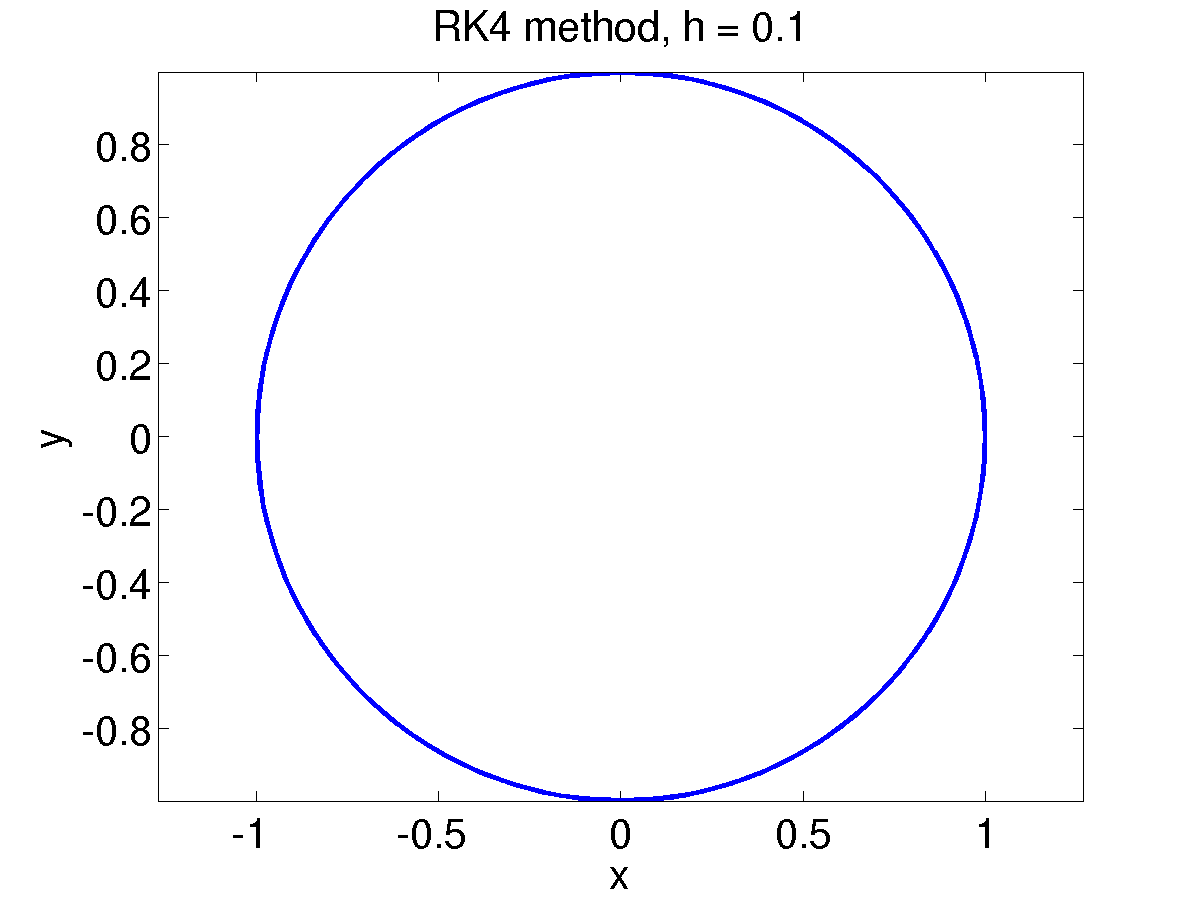
\includegraphics[height=0.5\textheight]{figures/RK4_1}
          \end{center}
        }
        \only<3|handout:1>
        {
          \begin{center}
            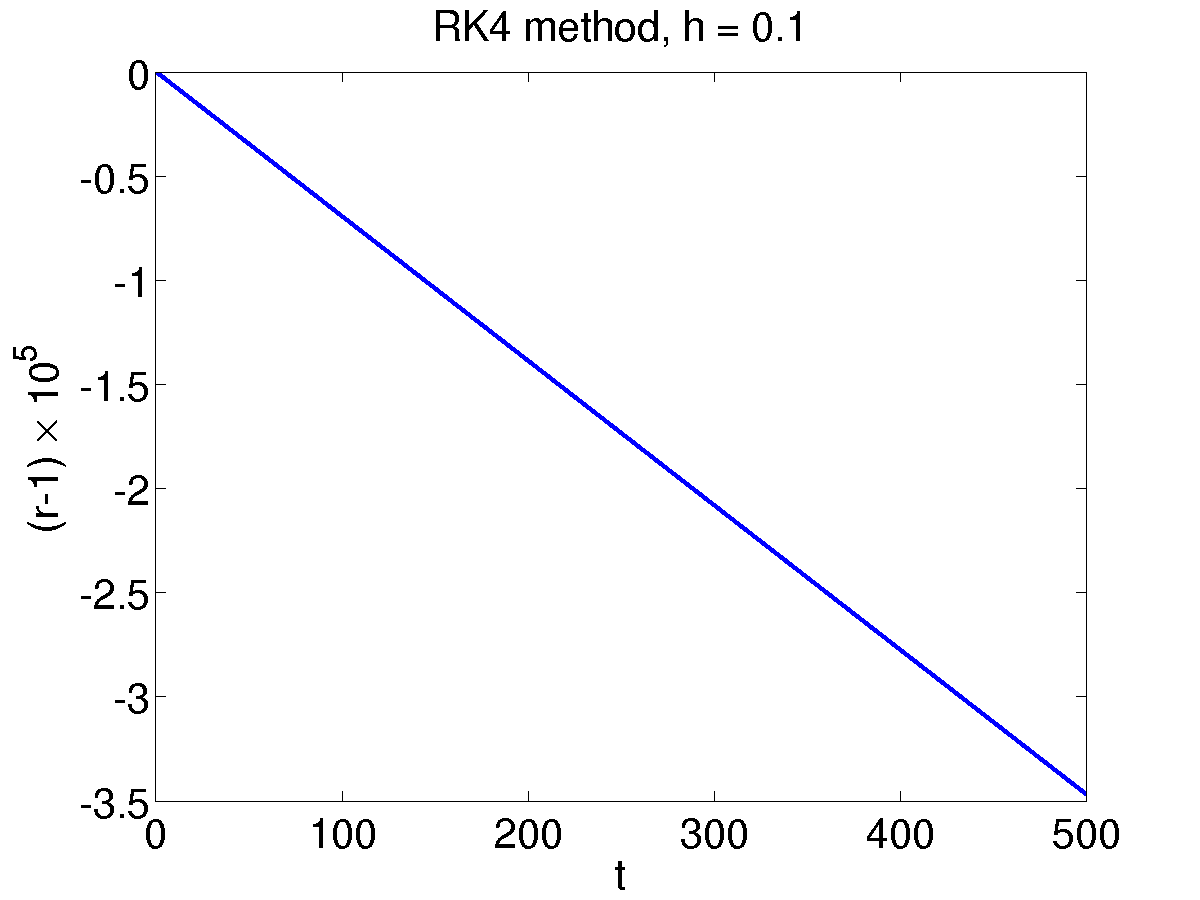
\includegraphics[height=0.5\textheight]{figures/RK4_rad1}
          \end{center}
        }
        \only<4|handout:0>
        {
          \begin{center}
            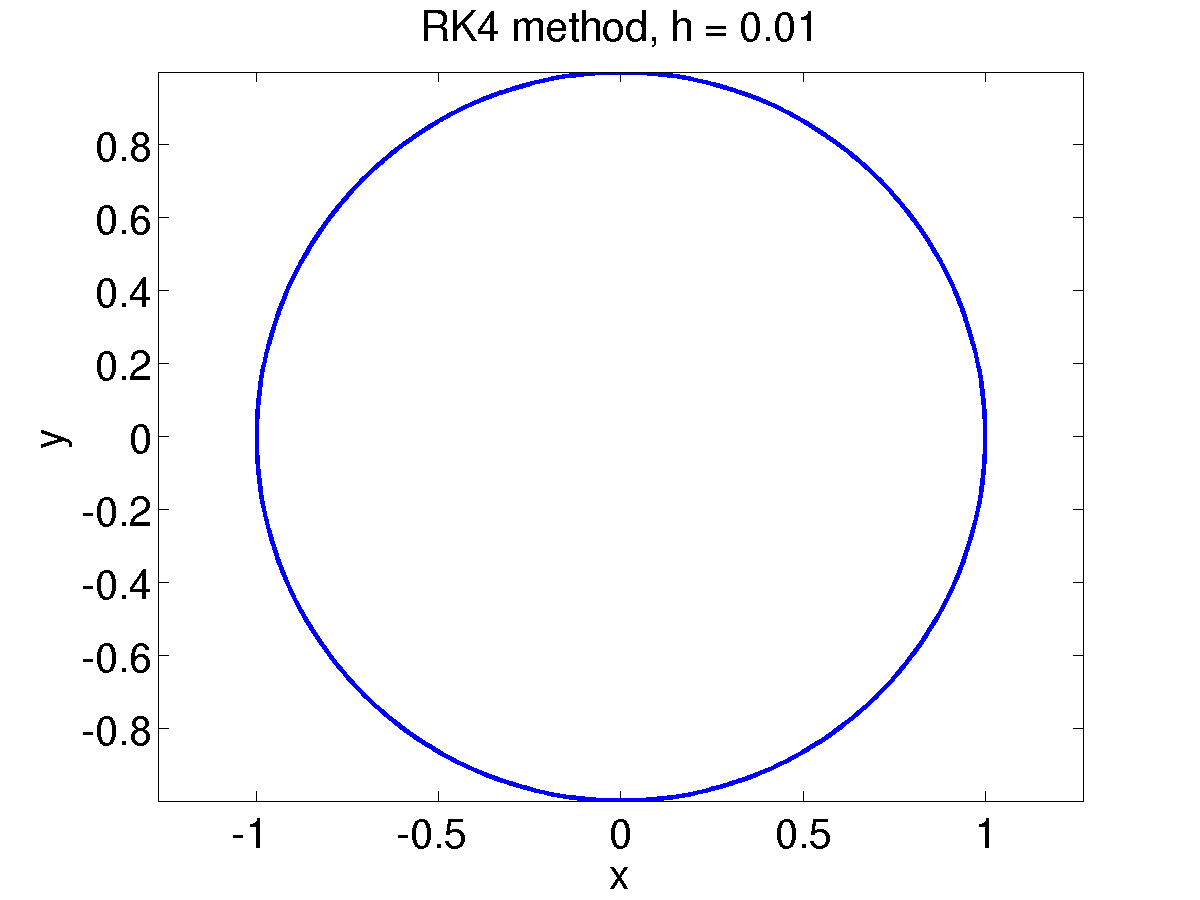
\includegraphics[height=0.5\textheight]{figures/RK4_2}
          \end{center}
        }
        \only<5|handout:2>
        {
          \begin{center}
            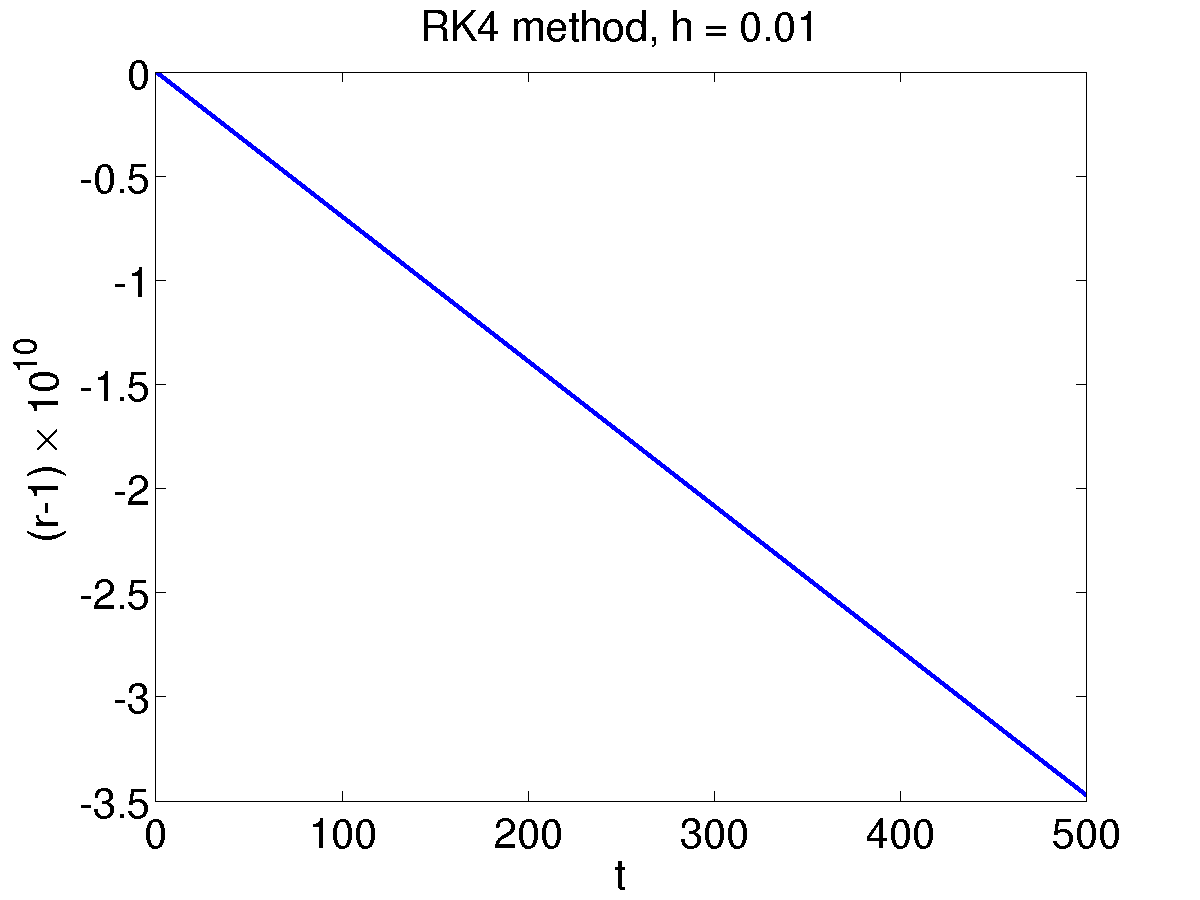
\includegraphics[height=0.5\textheight]{figures/RK4_rad2}
          \end{center}
        }
      \end{overlayarea}
    \end{column}
  \end{columns}

\end{frame}


\section{Summary}

\subsection{Summary}

\begin{frame}
  \frametitle{Summary}

  \begin{itemize}
  \item The errors at each step in an IVP solver are not independent.
    Hence the total error is not bounded by the sum of the local
    errors.
  \item If the local error is ${\cal O}(h^{n+1})$ then the global
    error is ${\cal O}(h^{n})$. Such a method is said to be of
    \emph{order $n$}.
  \item Euler's method has local error $\propto h^2$, hence global
    error $\propto h$.
  \item The Euler predictor-corrector method has local error $\propto
    h^3$, hence global error $\propto h^2$.
  \item \emph{Multistage} methods such as Runge-Kutta methods require
    only one known value $\by_{n}$ to start, and compute (many)
    estimates of the function $\bfm{f}$ for the algorithm to update
    $\by_{n+1}$.
  \item Runge-Kutta methods are the classic multistage methods; the
    predictor-corrector method is a second order RK method.
  \item RK4 is useful in practice.
  \end{itemize}

\end{frame}

\end{document}



%%% Local Variables:
%%% mode: latex
%%% TeX-master: t
%%% End:
